\chapter{Proposed software architecture}
\label{sec:Proposed software architecture}



% \section{Overview}



\section{System architecture choice}
We have chosen to utilise the \textbf{Model-View-Controller} system architecture, separating presentation and interaction from system data. 

\subsubsection{Advantages}
\begin{itemize}
	\item By keeping the visuals separated from the application data, we can achieve very loose coupling, as well as the ability to easily change the same data from many different views, for example via our desktop and web-based clients. \\
	\item If we ever need to change parts of the program, it will be easy to switch out parts of the code.
\end{itemize}


\subsubsection{Disadvantages}
\begin{itemize}
	\item We will most likely have a larger amount of classes than necessary for a project of this scope. \\
	\item The class hierarchy might become messier, as we will need a larger amount of classes for simple tasks.
\end{itemize}


\section{Subsystem decomposition}
We have grouped our classes into subsystems to create a clearer structure of the program. In this section, we will first show an overview of how the subsystems interact, and then a detailed look at the individual subsystems.

%insert subsystem diagrams here



\section{Hardware/software mapping}
\label{sec:Hardware/software mapping}
Below are the generalized components mapped to hardware or software
\begin{figure}[H]
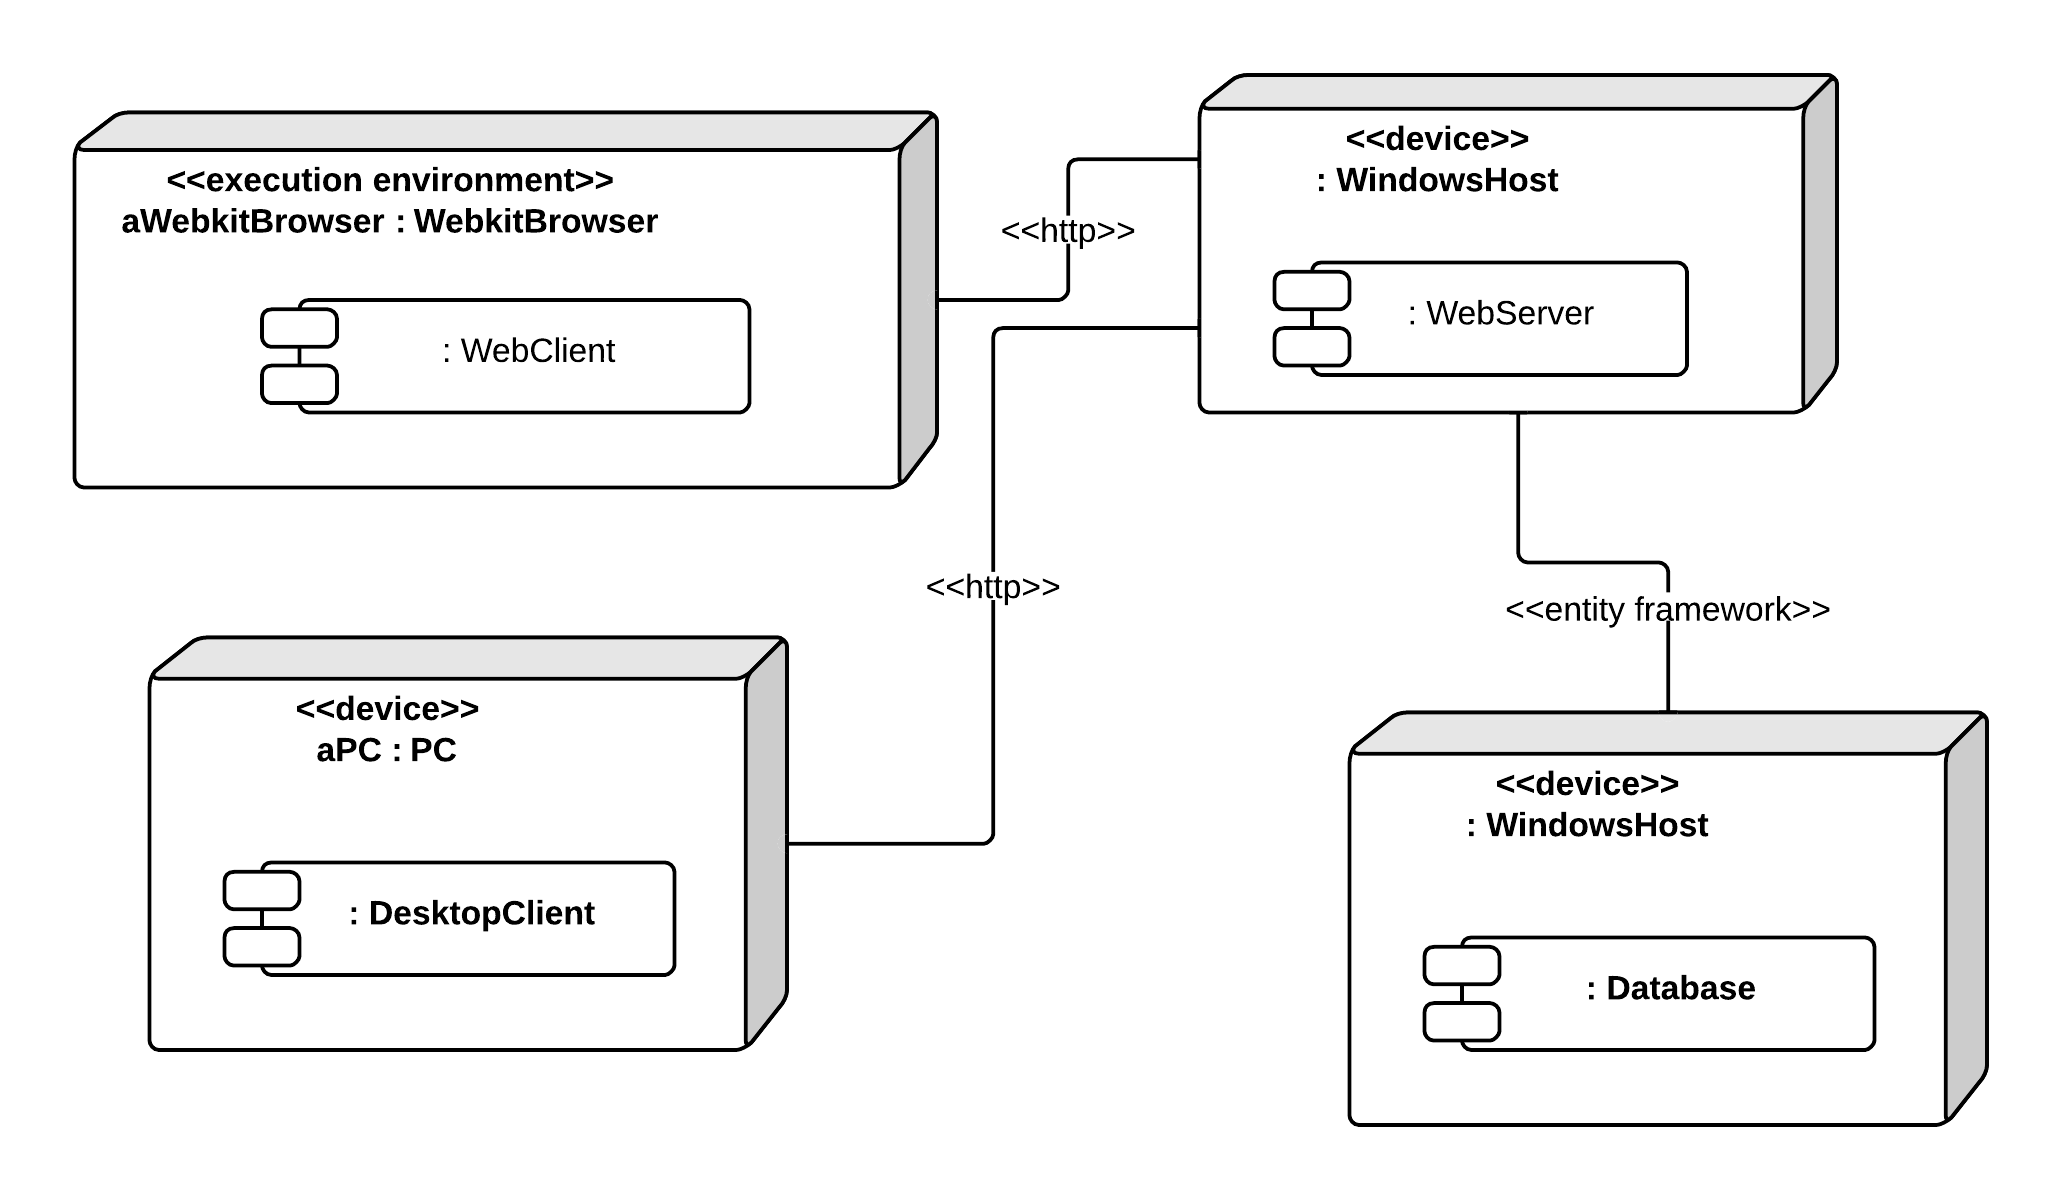
\includegraphics[scale=0.2]{img/SoftwareHardwareMapping.png}
\caption{Software/Hardware Mapping}
\label{fig:SoftwareHardwareMapping}
\end{figure}

\begin{itemize}
\item \textbf{aPC} is the hardware node for our DesktopClient component. The requirement it that it must run on a PC with Windows 7 or 8, utilizing .NET 4.5 or greater
\item \textbf{aWebkitBrowser} is a software environment implementing WebKit 2 or greater, able to execute our WebClient component. There are no requirements to the hardware platform
\item \textbf{WindowsHost} is the server hardware node. On it are two execution environments: .NET 4.5 or greater and MSSQL, required for our WebServer and Database components respectively. The components communicate by entity framework which allows for moving an environment and component to another WindowsHost hardware node.
\end{itemize}

\section{Persistent data management}

\subsection{RDBMS mapping}

\section{Access control and security}

\section{Global software control}
The global control flow is designed as procedure driven control flow with the use of threads to support concurrent users. When a user search for a movie a request is send from the web client and recieved by The WebServer. The WebServer receives the request and start a new thread that create a new RequestDelegater who process the request to Storage. If any, the Webserver receives the answer and send it to the webclient through the Communication Framework.

\section{Identifying services}
We have identified subsystem services for our program. They are shown in the figure below, and more detailed explanations for the services can be found beneath the diagram.

\begin{figure}[H]
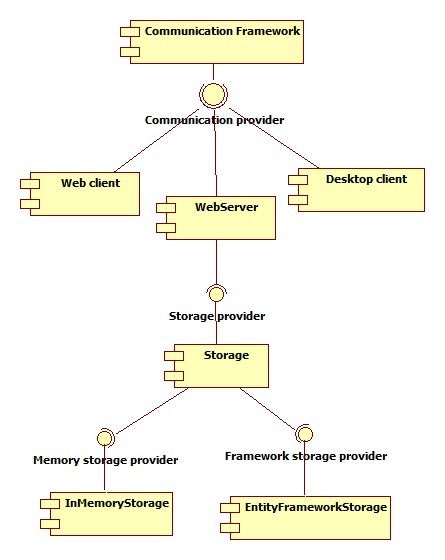
\includegraphics[scale=0.8]{img/SubsystemServices.jpg}
\caption{Software/Hardware Mapping}
\label{fig:Subsystem Services}
\end{figure}


\begin{itemize}
	\item Communication provider, which provides the clients and webserver with access to the communication framework, allowing them to send messages to each other.
	\item Storage provider, which provides the webserver with the methods required to get information / post information to the database.
	\item Framework storage provider, which provides the storage subsystem with the methods needed to store entities in-memory.
	\item Memory storage provider, which provides the storage subsystem with the methods required for storing entities via the entity framework.
\end{itemize}

\section{Boundary conditions}

We have indentified the following boundary conditions, and added them to the list of use cases in the RAD:

\begin{itemize}
	\item Start up and shutdown boundary use cases:
	\begin{itemize}
			\item StartWebServer
			\item ShutdownWebServer
			\item ConfigureWebServer
	\end{itemize}
	\item Exception use cases:
	\begin{itemize}
			\item ServerCrashException
			\item ConnectionLostException
	\end{itemize}
\end{itemize}

\section{Identifying optimization possibilities}